\documentclass[12pt]{article}
\usepackage{setspace, amsmath, mathdots, amssymb, graphicx, multirow, gensymb, slashbox, listings}
\usepackage[margin=1.5in]{geometry}
\onehalfspacing

\begin{document}

\noindent STA 250 HOMEWORK 2 \newline Yichuan Wang \newline \newline
Problem 1 \newline \newline
In this problem, we were assigned to use "Bag of Little Bootstraps" (BLB) algorithm to carry out bootstrapping on a rather large dataset and find out the standard errors of each coefficients. \newline
In the BLB algorithm, we first need to set parameters such as $s$ - number of unique subsets, $r$ - number of bootstrap datasets obtained from each subset, $\gamma$ - $b = n^\gamma$ is the size of each subset; in our case, we have $s = 5, r = 50, \gamma = 0.7$. Since the task will be divided into 250 jobs on Gauss cluster, we need to tackle the random number generation in order to have each 50 jobs sharing the same subset. It is easy to see that the solution is: after obtaining the subset index for each job, the random seed in that R session was set to be associated solely with such index; after subsetting from the whole dataset, the random seed was set to be related to the individual job index. In that way we first obtained only five subsets from the entire dataset, then for each subset, 50 different bootstrap datasets were generated. The algorithm worked quite efficiently with most jobs finishing in under ten minutes. The figure below shows standard errors for each of the 1000 estimated parameters obtained from bootstrap datasets: \newline
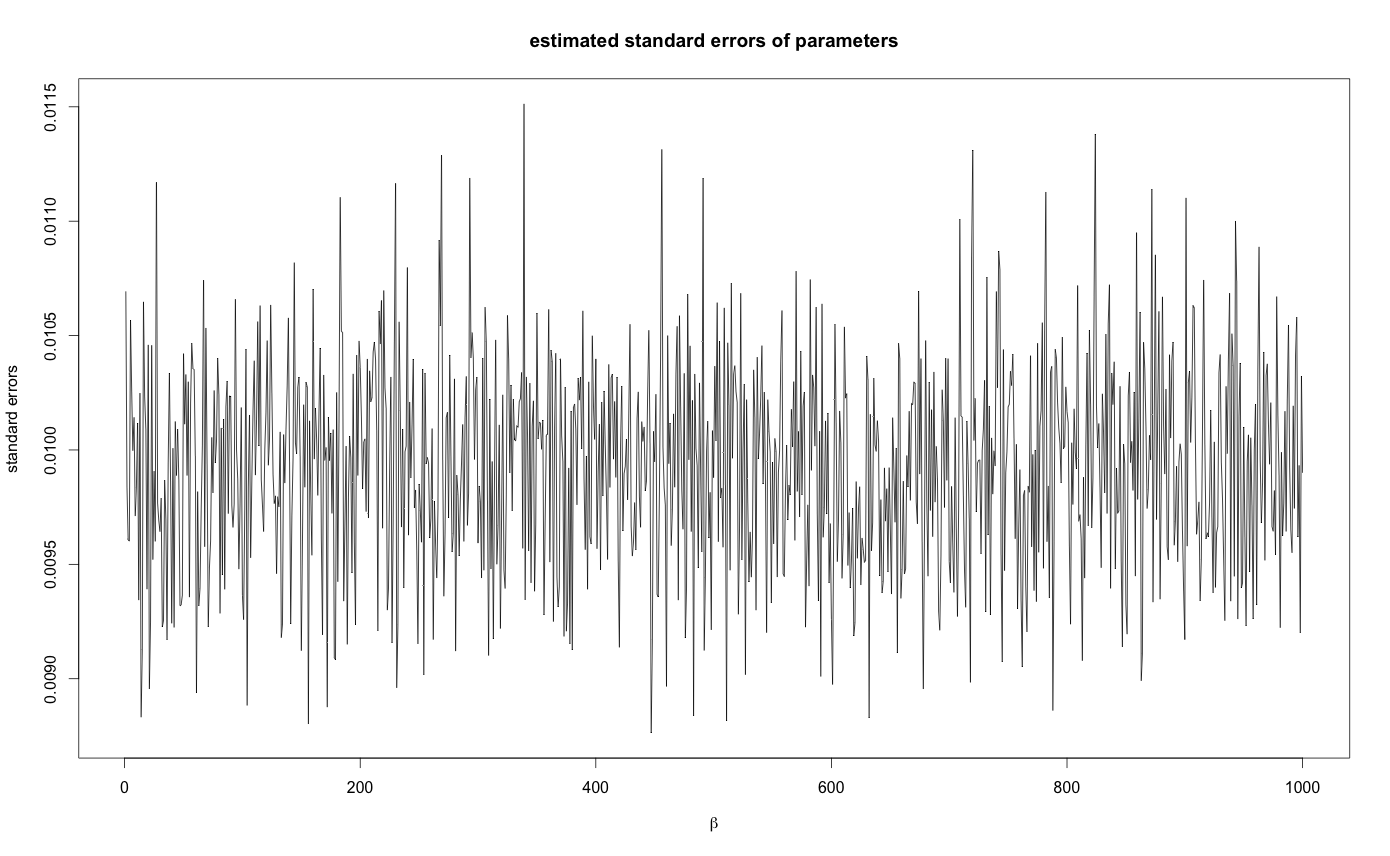
\includegraphics[width=\textwidth]{seplot.png} \newline
As seen in the graph, the standard errors varied about 0.01, which is expected in the instruction for this problem. \newline \newline
Problem 2 \newline \newline
In this problem, we used Python to carry out a MapReduce task on hadoop cluster of Amazon Web Serices (AWS). Firstly an Elastic MapReduce (EMR) cluster was created as instructed with one large master node and two large compute nodes. Data file was copied from the s3 bucket to "data" folder on HDFS. \newline
For the MapReduce procedure, the Map function reads each pair of $(x, y)$ and computes the lower, upper interval bounds for $x$ and $y$ individually, which four numbers form the key in the mapper output. The associated value/count with each key is set to be 1. Then the combination of keys and corresponding values is printed as output of the Map function. The Reduce function takes every combination of a key and a count; then starting from the second combination it reads, if the key is the same as the previous one, the associated count, i.e. 1, will be added to current count, otherwise the reducer will print out the previous key and count before setting the key and count to the newly read combination. Eventually after looping over all the input, the reducer needs to print out the last key and count. \newline
At first, my implementation was to have the Reduce function do all computing and the Map function simply print out its input. However it was not very efficient and somehow created output files weighing hundreds of megabytes. That implementation also somehow defies the purpose of MapReduce procedure since no mapping was really performed. The actual implementation gave much better performance, estimated to have finished within half an hour, and resulted in output files only weighing hundreds of kilobytes. Using the R script given, I obtained the following 2D histogram:
\begin{center}
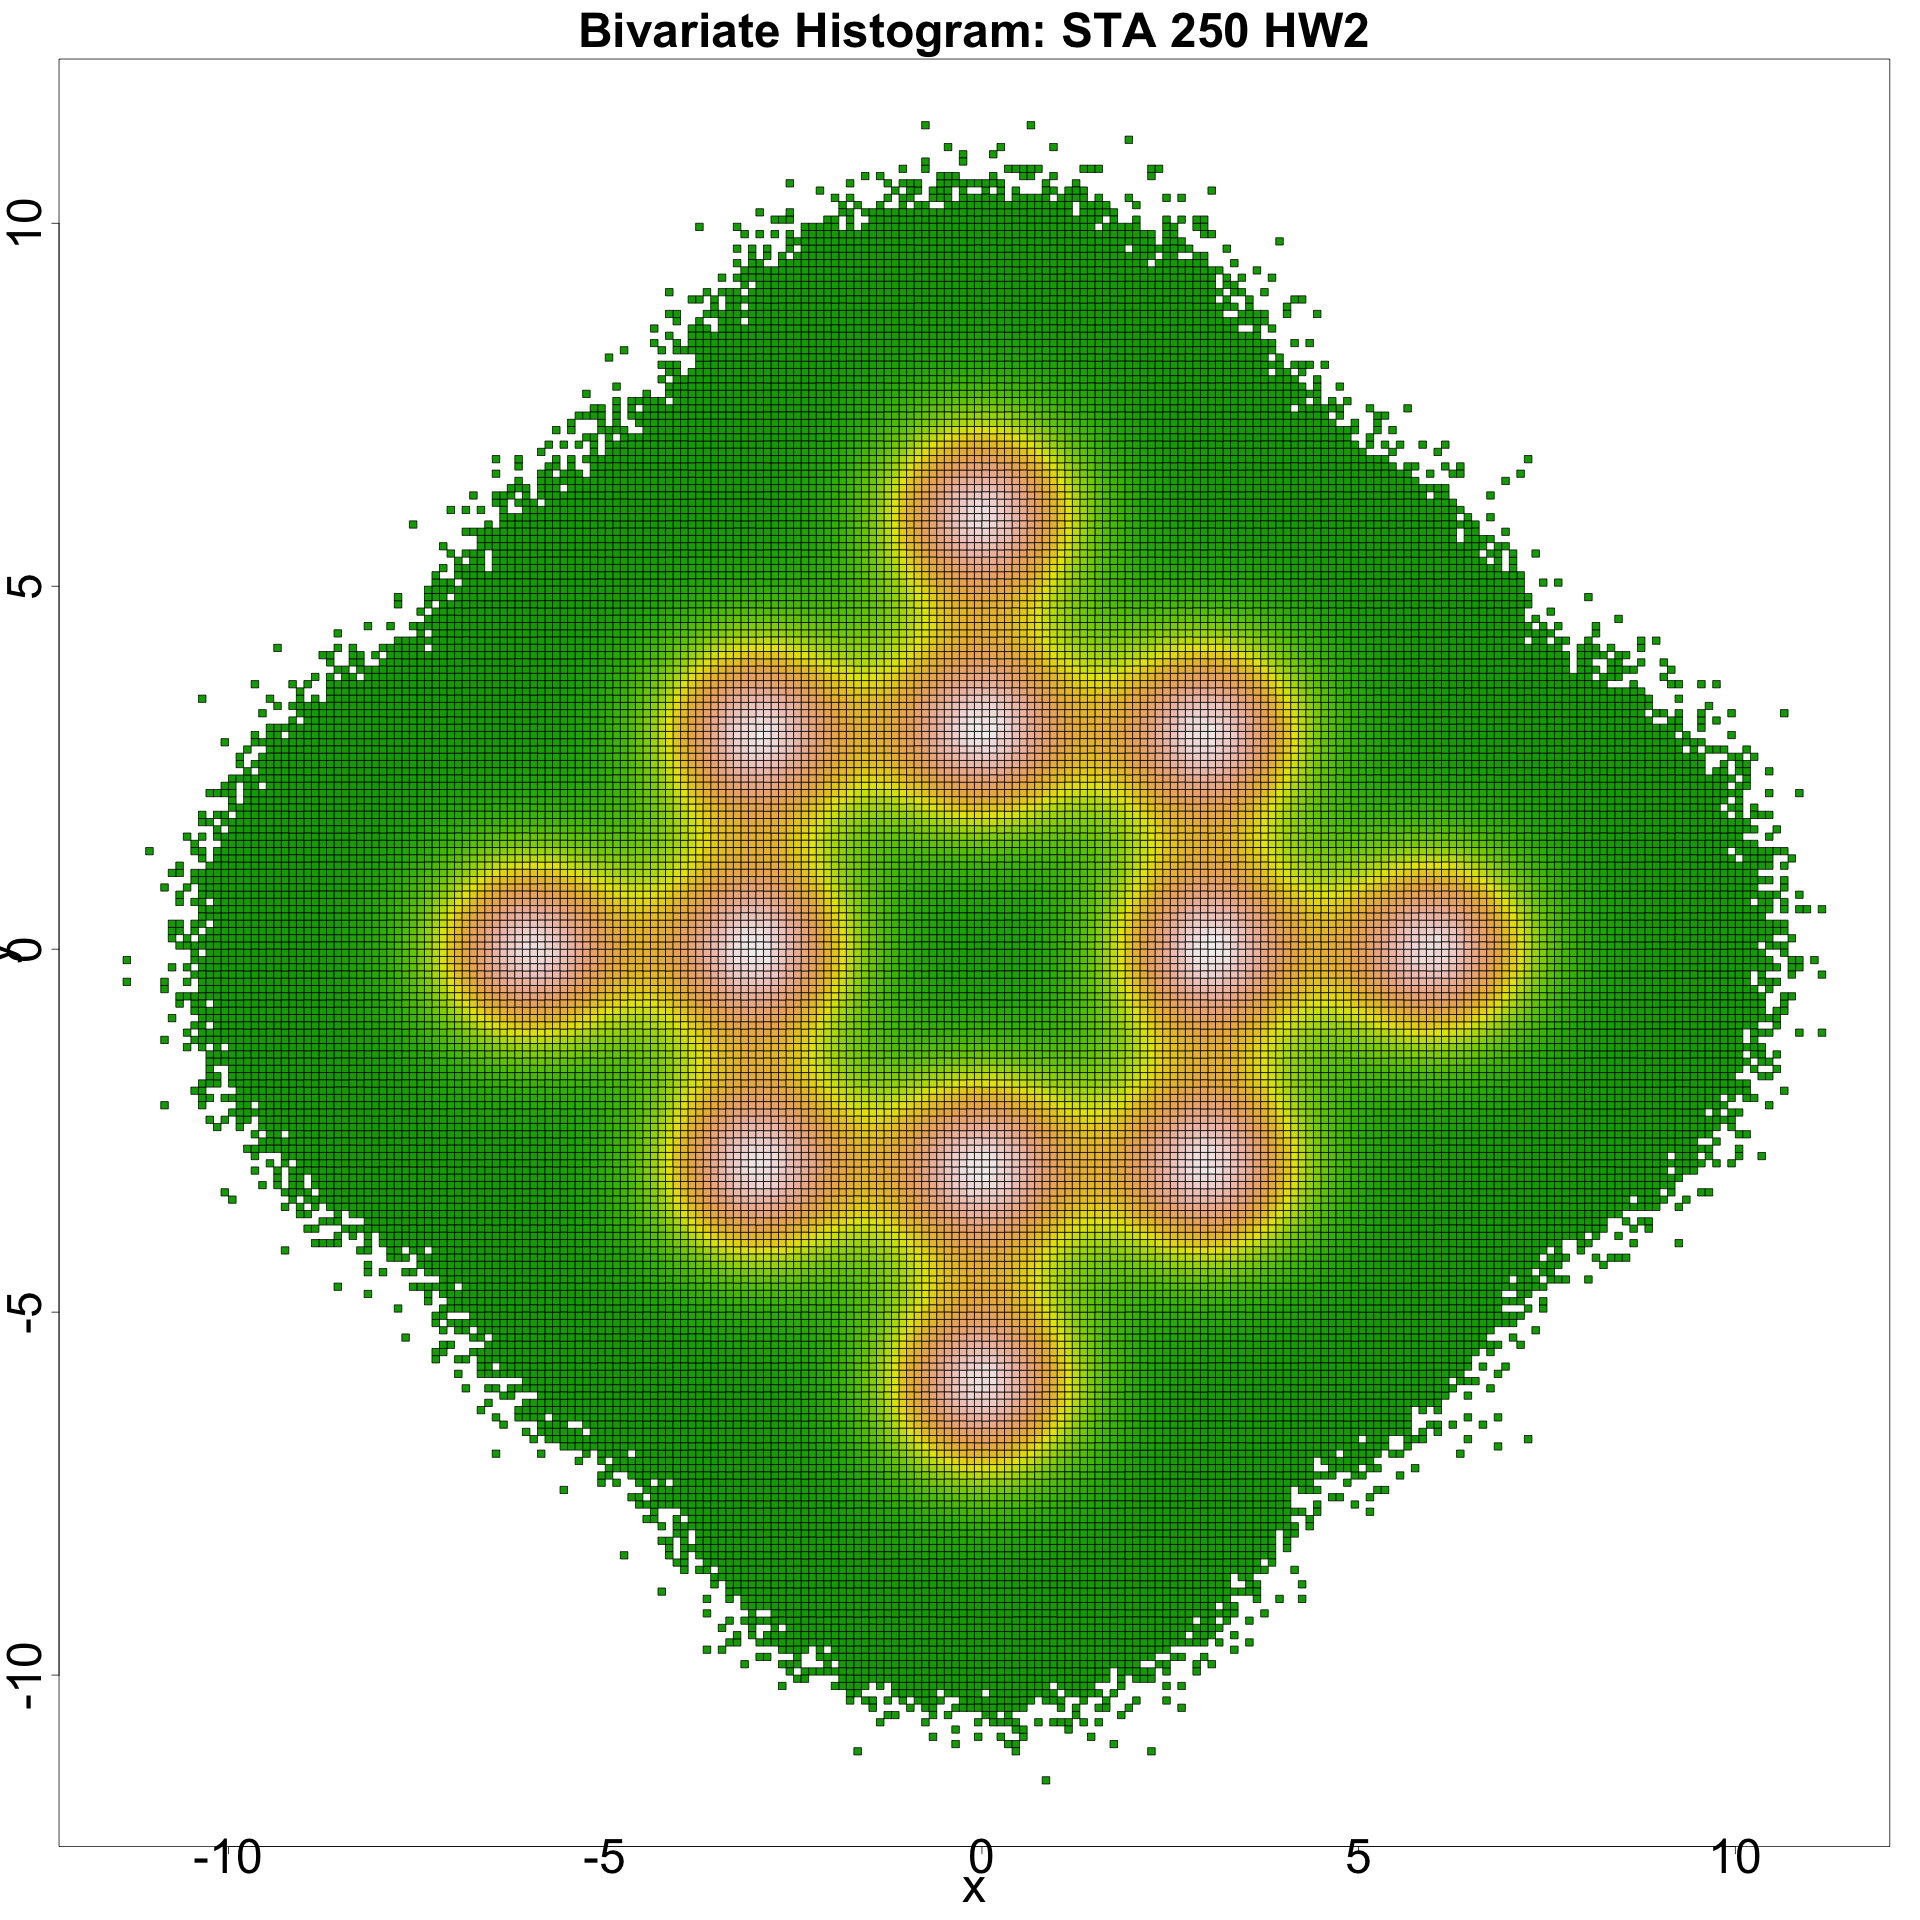
\includegraphics[width=0.95\textwidth]{hist2d.png}
\end{center}
Problem 3 \newline \newline
The cluster was set up as instructed in problem 2, and the data file was copied from s3 bucket to hadoop via the command:
\begin{lstlisting}
hadoop distcp s3://sta250bucket/groups.txt data/
\end{lstlisting}
Then in Hive, a two-column table named "groups" was created with the first column corresponding to group indices as string, the second to numerical values as double. Then the text file was read into the table by the command:
\begin{lstlisting}
LOAD DATA INPATH "data/groups.txt" INTO TABLE groups;
\end{lstlisting}
The within-group means and variances were calculated and exported into data/output directory using the following code:
\begin{lstlisting}
INSERT OVERWRITE DIRECTORY "data/output"
ROW FORMAT DELIMITED FIELDS TERMINATED BY ","
SELECT avg(v),variance(v) FROM groups GROUP BY g;
\end{lstlisting}
This would output the results into a file named "000000\_0" under the "output" directory; I converted it into a text file with shell command "cat". The within-group variances were plotted against the within-group means:
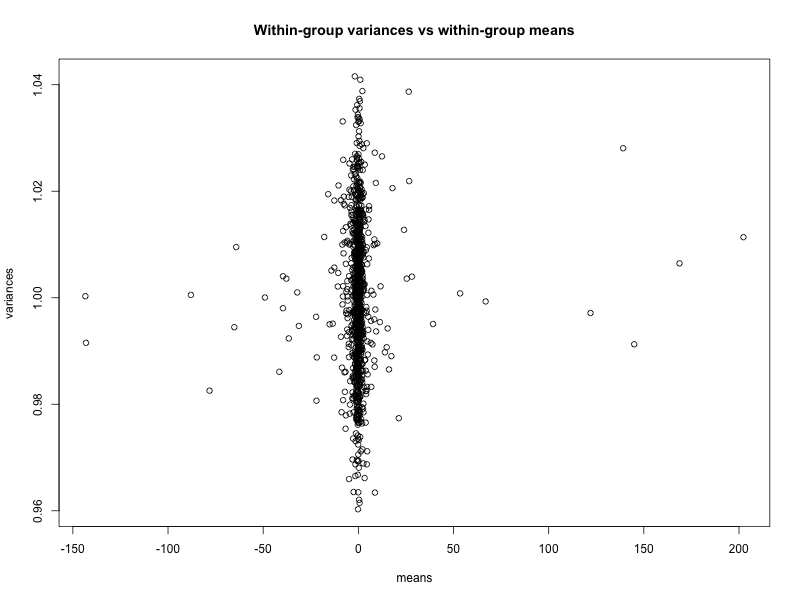
\includegraphics[width=\textwidth]{meanvar.png}
Since it was a quite simple task in this problem, it didn't take long to finish on Amazon cluster.

\end{document}
